\appendix
\renewcommand{\appendixname}{APPENDIX}
\captionsetup[table]{labelfont=bf,name=Table\space,labelsep=space}
\captionsetup[figure]{labelfont=bf,name=Figure\space,labelsep=space}
\renewcommand\thefigure{\thechapter\arabic{figure}} 
\newcommand{\stoptocwriting}{%
  \addtocontents{toc}{\protect\setcounter{tocdepth}{-5}}}
\newcommand{\resumetocwriting}{%
  \addtocontents{toc}{\protect\setcounter{tocdepth}{\arabic{tocdepth}}}}

\captionsetup{
  singlelinecheck=false,
  % textfont=bf
}

\newpage
\phantomsection
\addcontentsline{toc}{chapter}{\bf APPENDICES}
\begin{center}
    \vspace*{\fill}
    \large{\bf APPENDICES}
    \vspace*{\fill}
\end{center}
\newpage

\phantomsection
\addcontentsline{toc}{section}{APPENDIX A: Time domain and Frequency domain plots}
\section*{APPENDIX A: Time domain and Frequency domain plots}
\stoptocwriting
\begin{figure}[htbp]
\caption{STFT plot of character A flickering at 8Hz frequency}
\label{fig:stft_8Hz}
\centering

    \subfloat[Fz]{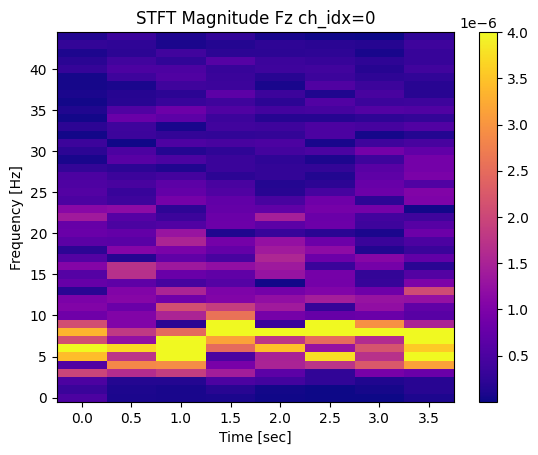
\includegraphics[width=0.4\textwidth]{figures/8Hz_PSD/stft_plot0_8Hz.png}\label{fig:stft_8Hz_fz}}
    \hfill
    \subfloat[C3]{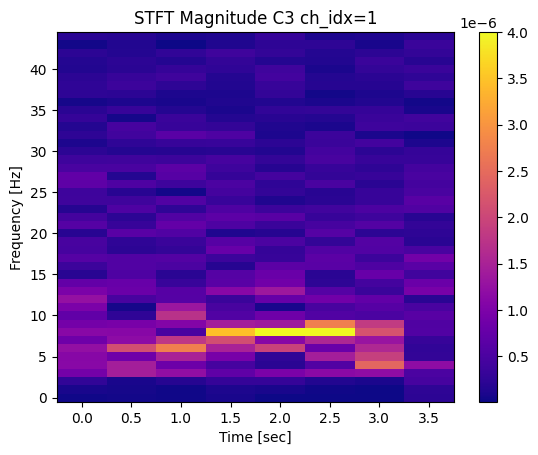
\includegraphics[width=0.4\textwidth]{figures/8Hz_PSD/stft_plot1_8Hz.png}\label{fig:stft_8Hz_c3}}
    
    \vspace{0.5cm}
    
    \subfloat[Cz]{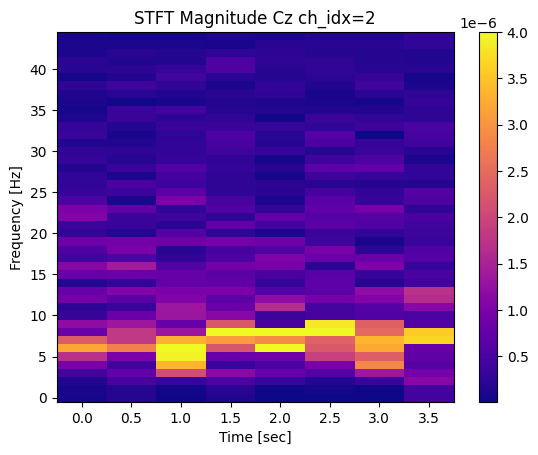
\includegraphics[width=0.4\textwidth]{figures/8Hz_PSD/stft_plot2_8Hz.png}\label{fig:stft_8Hz_cz}}
    \hfill
    \subfloat[C4]{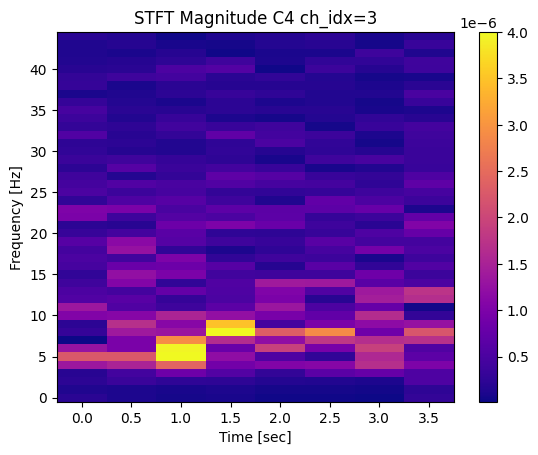
\includegraphics[width=0.4\textwidth]{figures/8Hz_PSD/stft_plot3_8Hz.png}\label{fig:stft_8Hz_c4}}
    
    \vspace{0.5cm}
    
    \subfloat[Pz]{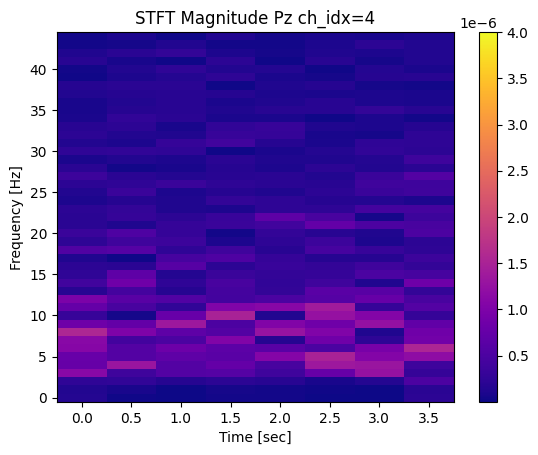
\includegraphics[width=0.4\textwidth]{figures/8Hz_PSD/stft_plot4_8Hz.png}\label{fig:stft_8Hz_pz}}
    \hfill
    \subfloat[PO7]{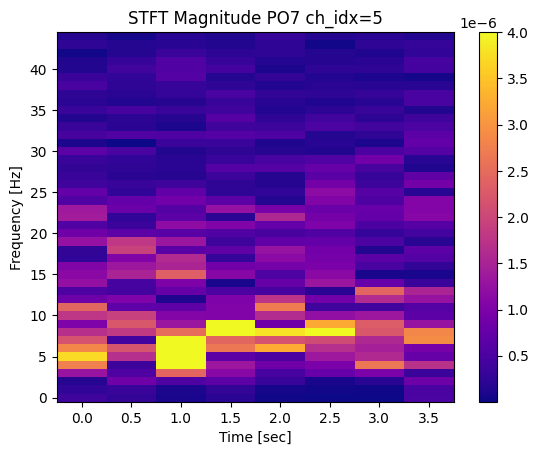
\includegraphics[width=0.4\textwidth]{figures/8Hz_PSD/stft_plot5_8Hz.png}\label{fig:stft_8Hz_po7}}
    
    \vspace{0.5cm}
    
    \subfloat[Oz]{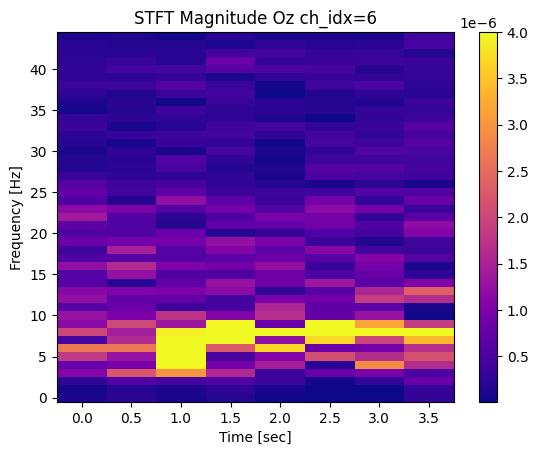
\includegraphics[width=0.4\textwidth]{figures/8Hz_PSD/stft_plot6_8Hz.png}\label{fig:stft_8Hz_oz}}
    \hfill
    \subfloat[PO8]{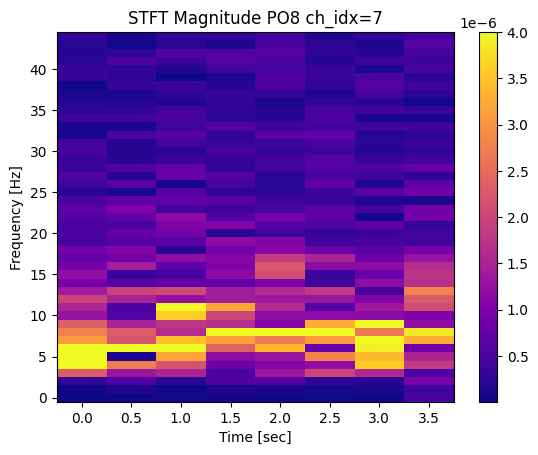
\includegraphics[width=0.4\textwidth]{figures/8Hz_PSD/stft_plot7_8Hz.png}\label{fig:stft_8Hz_po8}}

\end{figure}


\begin{figure}[htbp]
    \caption{STFT plot of character A flickering at 9Hz frequency}
    \label{fig:stft_9Hz}
    \centering

    \subfloat[Fz]{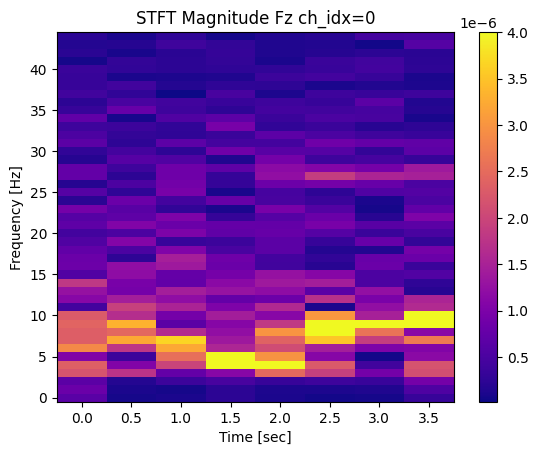
\includegraphics[width=0.4\textwidth]{figures/9Hz_PSD/stft_plot0_9Hz.png}\label{fig:stft_9Hz_fz}}
    \hfill
    \subfloat[C3]{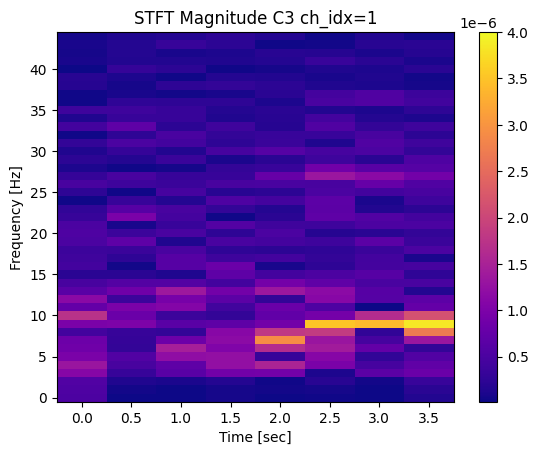
\includegraphics[width=0.4\textwidth]{figures/9Hz_PSD/stft_plot1_9Hz.png}\label{fig:stft_9Hz_c3}}

    \vspace{0.5cm}

    \subfloat[Cz]{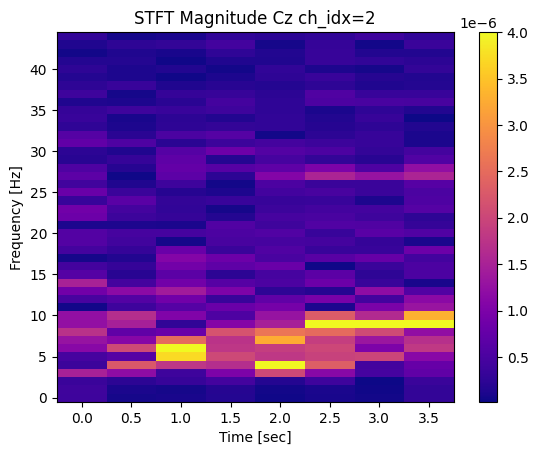
\includegraphics[width=0.4\textwidth]{figures/9Hz_PSD/stft_plot2_9Hz.png}\label{fig:stft_9Hz_cz}}
    \hfill
    \subfloat[C4]{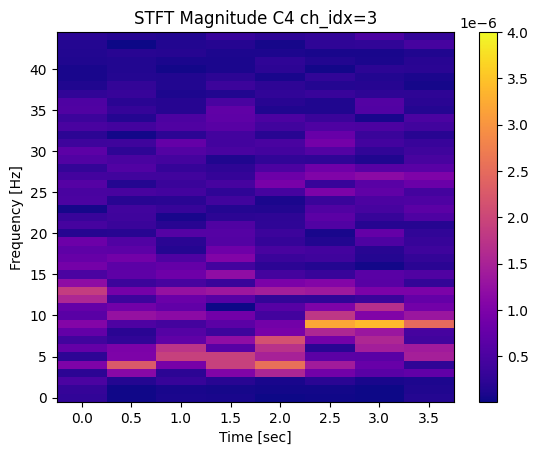
\includegraphics[width=0.4\textwidth]{figures/9Hz_PSD/stft_plot3_9Hz.png}\label{fig:stft_9Hz_c4}}

    \vspace{0.5cm}

    \subfloat[Pz]{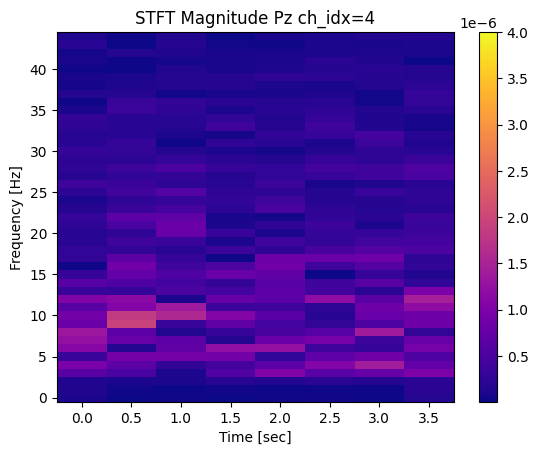
\includegraphics[width=0.4\textwidth]{figures/9Hz_PSD/stft_plot4_9Hz.png}\label{fig:stft_9Hz_pz}}
    \hfill
    \subfloat[PO7]{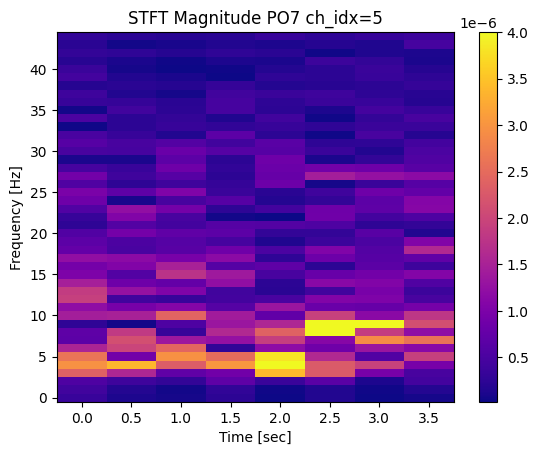
\includegraphics[width=0.4\textwidth]{figures/9Hz_PSD/stft_plot5_9Hz.png}\label{fig:stft_9Hz_po7}}

    \vspace{0.5cm}

    \subfloat[Oz]{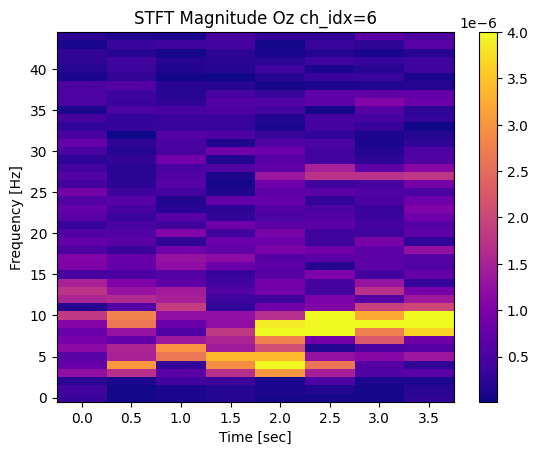
\includegraphics[width=0.4\textwidth]{figures/9Hz_PSD/stft_plot6_9Hz.png}\label{fig:stft_9Hz_oz}}
    \hfill
    \subfloat[PO8]{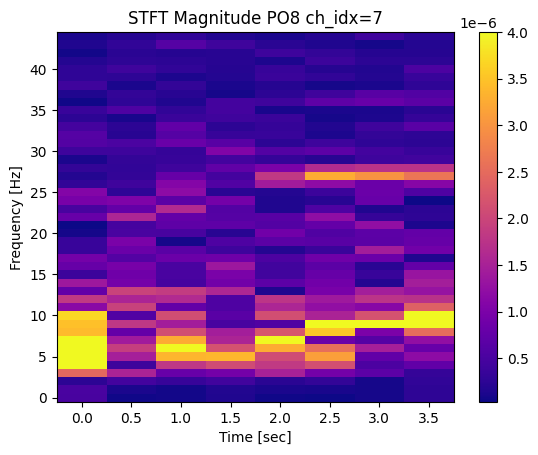
\includegraphics[width=0.4\textwidth]{figures/9Hz_PSD/stft_plot7_9Hz.png}\label{fig:stft_9Hz_po8}}
\end{figure}


\begin{figure}[htbp]
    \caption{Frequency and waveform plot of each subspeller of participant S8}
    \label{fig:freq_best_participant}
    \centering
    \subfloat[subspeller 1]{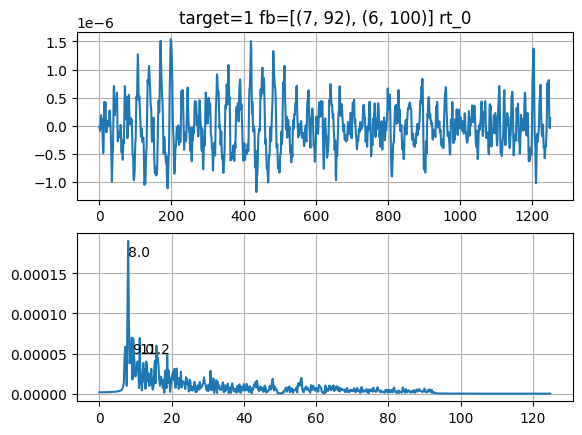
\includegraphics[width=0.4\textwidth]{figures/best_participant_rts/target1_plot.png}\label{fig:freq_best_subspeller1}}
    \hfill
    \subfloat[subspeller 2]{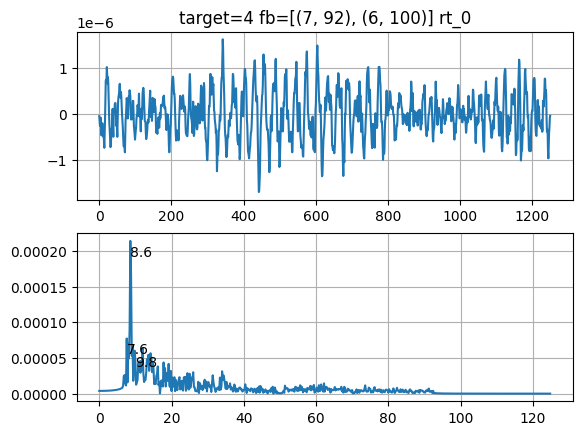
\includegraphics[width=0.4\textwidth]{figures/best_participant_rts/target4_plot.png}\label{fig:freq_best_subspeller2}}

    \vspace{0.5cm}

    \subfloat[subspeller 3]{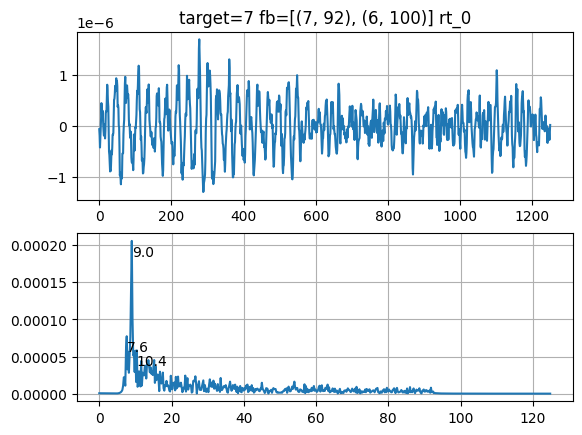
\includegraphics[width=0.4\textwidth]{figures/best_participant_rts/target7_plot.png}\label{fig:freq_best_subspeller3}}
    \hfill
    \subfloat[subspeller 4]{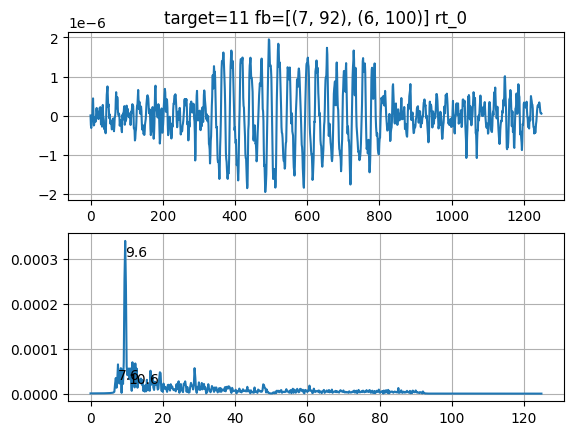
\includegraphics[width=0.4\textwidth]{figures/best_participant_rts/target11_plot.png}\label{fig:freq_best_subspeller4}}
\end{figure}


\begin{figure}[htbp]
    \caption{Frequency and waveform plot of each subspeller of participant S4}
    \label{fig:freq_worst_participant}
    \centering
    \subfloat[subspeller 1]{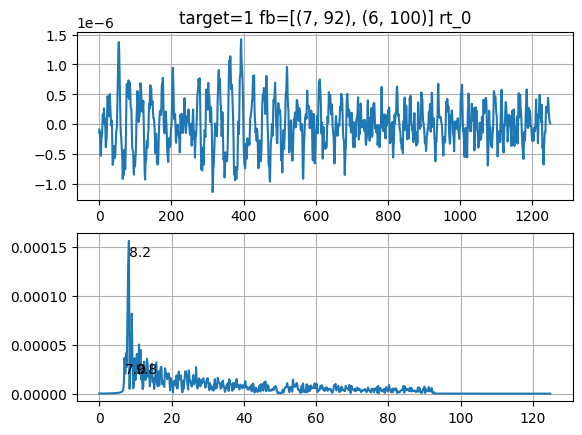
\includegraphics[width=0.4\textwidth]{figures/worst_participant_rts/target1_plot.png}\label{fig:freq_worst_subspeller1}}
    \hfill
    \subfloat[subspeller 2]{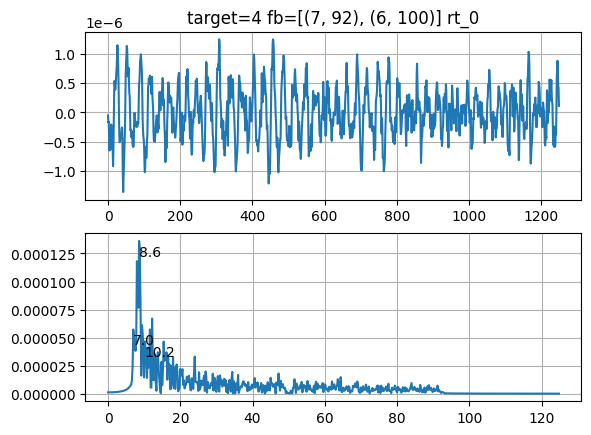
\includegraphics[width=0.4\textwidth]{figures/worst_participant_rts/target4_plot.png}\label{fig:freq_worst_subspeller2}}

    \vspace{0.5cm}

    \subfloat[subspeller 3]{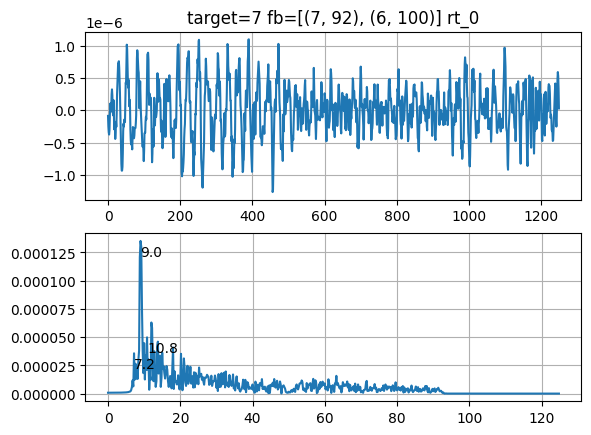
\includegraphics[width=0.4\textwidth]{figures/worst_participant_rts/target7_plot.png}\label{fig:freq_worst_subspeller3}}
    \hfill
    \subfloat[subspeller 4]{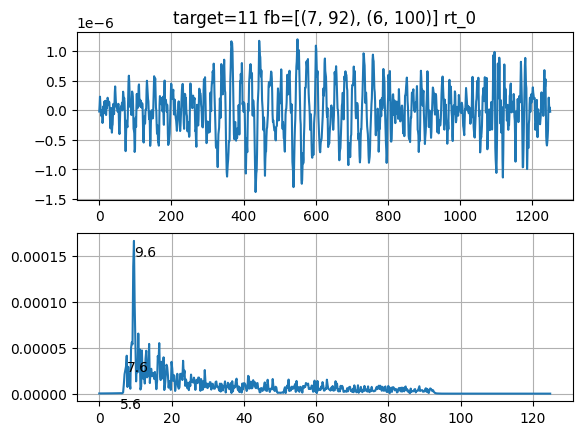
\includegraphics[width=0.4\textwidth]{figures/worst_participant_rts/target11_plot.png}\label{fig:freq_worst_subspeller4}}
\end{figure}


\resumetocwriting

